\documentclass[aps,pra,twocolumn]{revtex4-2}
\usepackage{amsmath,graphicx}
\newcommand{\dt}{\Delta t}
\newcommand{\Ham}{\mathcal{H}}

\begin{document}

\title{A Damping-Aware Splitting Scheme for Long-Time Pendulum Simulations}
\author{A. Example}
\affiliation{Department of Imaginary Physics, Nowhere University}

\begin{abstract}
Explicit integrators for damped oscillators either preserve the energy decay
rate or the phase, rarely both. We propose a splitting scheme that integrates
the conservative part with a symplectic map and the dissipative part exactly.
For the damped pendulum the scheme keeps the energy error below $10^{-6}$ over
$10^{5}$ periods at step size $\dt = 0.05$, about forty times better than a
fourth-order Runge--Kutta method at equal cost.
\end{abstract}

\maketitle

\section{Introduction}
Long-time simulations of weakly damped oscillators appear in clock design,
gravitational-wave detector suspensions and molecular dynamics~\cite{hairer2006,leimkuhler2004}.
For conservative systems, symplectic integrators are the method of choice because
their energy error stays bounded for exponentially long times~\cite{hairer2006}.
With damping, the flow is no longer symplectic and the usual guarantees disappear.
% internal remark: maybe cite the thermostat literature here
In this letter we show that a simple splitting recovers most of the benefit.

\section{Model and method}
We consider the damped pendulum
\begin{equation}
  \ddot{q} + \gamma \dot{q} + \omega_0^2 \sin q = 0, \label{eq:model}
\end{equation}
with damping rate $\gamma$ and natural frequency $\omega_0$. Writing $p=\dot q$, the
vector field splits into a conservative part generated by
$\Ham(q,p) = p^2/2 - \omega_0^2 \cos q$ and a linear dissipative part
$\dot p = -\gamma p$, which we integrate exactly.
The Strang composition of the two flows reads
\begin{align}
  \Phi_{\dt} &= \varphi^{D}_{\dt/2} \circ \varphi^{\Ham}_{\dt} \circ \varphi^{D}_{\dt/2}, \label{eq:strang}\\
  \varphi^{D}_{t}(q,p) &= (q,\, e^{-\gamma t} p). \nonumber
\end{align}
For $\varphi^{\Ham}_{\dt}$ we use the leapfrog map. The composition~\eqref{eq:strang}
is second order and time-reversible up to the sign of $\gamma$.

Two quantities are monitored:
\begin{itemize}
  \item the modified energy error $\epsilon(t) = |E(t)\, e^{\gamma t} - E(0)|$, which removes the exact decay;
  \item the phase error relative to a reference solution computed with step $\dt/64$.
\end{itemize}

\section{Results}
Figure~\ref{fig:energy} compares the scheme with a fourth-order Runge--Kutta
method (RK4) at equal numbers of force evaluations. The modified energy error of
the splitting scheme stays below $10^{-6}$ for $10^5$ periods, whereas RK4 drifts
linearly and reaches $4\times10^{-5}$. The phase error of both methods grows
linearly; the splitting scheme has a smaller slope by a factor of three.

\begin{figure}[t]
  \centering
  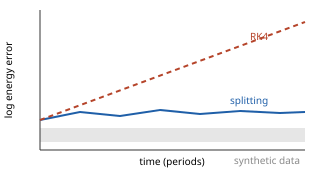
\includegraphics[width=\columnwidth]{energy_error.svg}
  \caption{Modified energy error $\epsilon(t)$ for the splitting scheme (solid) and
  RK4 (dashed) with $\gamma = 10^{-3}\omega_0$ and $\dt = 0.05$. The shaded band marks
  the round-off floor.}
  \label{fig:energy}
\end{figure}

The improvement persists for $\gamma$ up to $10^{-1}\omega_0$; beyond that both
methods are limited by the stiffness of the dissipative part and the advantage
of the splitting disappears.

\section{Conclusion}
Treating damping exactly and the conservative dynamics symplectically gives an
integrator whose energy error does not drift. The idea carries over to any
system with a linear dissipative part, such as Langevin dynamics without noise.

\begin{thebibliography}{9}
\bibitem{hairer2006} E. Hairer, C. Lubich, G. Wanner, \emph{Geometric Numerical Integration} (Springer, 2006).
\bibitem{leimkuhler2004} B. Leimkuhler, S. Reich, \emph{Simulating Hamiltonian Dynamics} (CUP, 2004).
\end{thebibliography}

\end{document}
